\section{Ejercicio 2}
\label{sec:ej2}

\subsection{Consigna}

\begin{enumerate}
	\item[\textbf{a)}] Comprobar estadísticamente la capacidad de la red de Hopfield '82 calculando la cantidad máxima de patrones pseudo-aleatorios aprendidos en función del tamaño de la red. Obtener experimentalmente los resultados del Cuadro \ref{tab:teorica_hertz} (los valores del cuadro corresponden a una iteración con actualización sincrónica).
	
	\begin{table}[htbp]
		\centering
		\begin{tabular}{cc}
			\toprule
			\textbf{$P_{\text{error}}$} & \textbf{$p_{\text{max}}/N$} \\
			\midrule
			0,001 & 0,105 \\
			0,0036 & 0,138 \\
			0,01 & 0,185 \\
			0,05 & 0,37 \\
			0,1 & 0,61 \\
			\bottomrule
		\end{tabular}
		\caption{Valores teóricos de probabilidad de error y capacidad límite (Tabla 2.1, sección 2.2, Hertz, Krogh \& Palmer, pág. 19).}
		\label{tab:teorica_hertz}
	\end{table}
	
	\item[\textbf{b)}] Proponga una manera de generar patrones con distintos grados de correlación. Utilice el método propuesto para analizar cómo varía la capacidad de la red de Hopfield en función de la correlación entre patrones.
\end{enumerate}

\subsection{Resolución}

\subsubsection{Metodología experimental para patrones descorrelacionados}
\label{subsec:metodologia_ej2}

Para obtener experimentalmente los valores de capacidad requeridos en la Tabla 2.1 mencionada en la consigna, se diseñó un algoritmo que evalúa la probabilidad de error empírica de la red tras un único paso de actualización. El procedimiento computacional implementado consistió en los siguientes pasos:

\begin{enumerate}
	\item \textbf{Generación de patrones:} Se generó un conjunto de $p$ patrones $\xi^\mu$ de dimensión $N$. Para garantizar la independencia estadística requerida por el modelo, cada componente $\xi_i^\mu \in \{-1, 1\}$ fue extraída de una distribución uniforme discreta con una probabilidad de $0.5$ para cada estado.
	
	\item \textbf{Entrenamiento:} Se construyó la matriz de pesos sinápticos $w_{ij}$ aplicando la regla de Hebb sobre los $p$ patrones generados.
	
	\item \textbf{Actualización sincrónica:} Se presentó cada uno de los patrones originales $\xi^\mu$ como estado inicial de la red. A continuación, se aplicó \textbf{exactamente una iteración con actualización sincrónica}, recalculando el estado de las $N$ neuronas de manera simultánea.
	
	\item \textbf{Cálculo de error global empírico:} Tras la actualización, se contabilizó la cantidad de bits que diferían de su estado original. La tasa de error experimental de la red ($E_{total}$) se calculó como la sumatoria de todos los bits erróneos dividida por la cantidad total de bits evaluados ($p \times N$).
	
	\item \textbf{Determinación de la capacidad:} Para cada umbral de tolerancia teórica $P_{error}$ establecido por la consigna (ej. $0.01$, $0.05$, etc.), se incrementó iterativamente la cantidad de patrones almacenados $p$. Se definió a $p_{max}$ como la cantidad máxima de patrones que la red logró procesar cumpliendo la condición de que $E_{total} \leq P_{error}$. Finalmente, la capacidad límite para cada umbral se reportó mediante la relación $p_{max}/N$.
\end{enumerate}

Fue entonces de esa manera que se corrieron 10 ensayos para cada valor $P_{error}$ y así calcular la capacidad promediandolos. Los resultados se pueden observar en el Cuadro \ref{tab:resultados_ej2}. Se observa como a medida que el umbral de error se hace más permisivo, la red es capaz de recordar más cantidad de patrones. Por otro lado, se puede ver la similitud con los valores teóricos del Cuadro \ref{tab:teorica_hertz}. En conclusión, se puede decir que se pudo reproducir la tabla teórica exitosamente.

\begin{table}[htbp]
	\centering
	\begin{tabular}{cc}
		\toprule
		\textbf{$P_{error}$ (Objetivo)} & \textbf{Capacidad Promedio ($p_{max}/N$)} \\
		\midrule
		0.001  & 0.1100 \\
		0.0036 & 0.1400 \\
		0.01   & 0.1900 \\
		0.05   & 0.3633 \\
		0.1    & 0.6167 \\
		\bottomrule
	\end{tabular}
	\caption{Resultados experimentales de la capacidad límite de la red en función de la probabilidad de error tolerada.}
	\label{tab:resultados_ej2}
\end{table}

\subsection{Generación de patrones correlacionados}
\label{subsec:patrones_correlacionados}

Para evaluar el impacto de la correlación espacial en la capacidad de la red, se implementó un algoritmo basado en la generación de una familia de patrones a partir de un ancestro común. Sea $\xi^M \in \{-1, 1\}^N$ un ``patrón madre'' generado de forma puramente aleatoria (donde cada estado tiene probabilidad $0.5$). 

A partir de este patrón madre, se genera un conjunto de $p$ patrones descendientes (\textit{offsprings}) $\xi^\mu$. Cada componente $i$ de un patrón descendiente se obtiene multiplicando la componente original del patrón madre por una máscara de mutación estocástica $m_i^\mu$:
\begin{equation}
	\xi_i^\mu = \xi_i^M \cdot m_i^\mu
\end{equation}

La variable aleatoria $m_i^\mu \in \{-1, 1\}$ determina si el bit se mantiene idéntico al patrón madre ($m_i^\mu = 1$) o si se invierte ($m_i^\mu = -1$). Definimos la probabilidad de inversión (\textit{flip}) como $P(m_i^\mu = -1) = p_{flip}$. En consecuencia, el valor esperado de la máscara de mutación para cualquier componente es:
\begin{equation}
	E[m_i^\mu] = (1) \cdot P(m_i^\mu = 1) + (-1) \cdot P(m_i^\mu = -1) = (1 - p_{flip}) - p_{flip} = 1 - 2p_{flip}
\end{equation}

El objetivo es que cualquier par de patrones descendientes distintos, digamos $\xi^\mu$ y $\xi^\nu$ (con $\mu \neq \nu$), posean un nivel de correlación $C$ esperado entre sí. La correlación espacial teórica se define como el valor esperado del producto de sus componentes:
\begin{equation}
	C = E[\xi_i^\mu \xi_i^\nu] = E[(\xi_i^M m_i^\mu) (\xi_i^M m_i^\nu)]
\end{equation}

Dado que para cualquier estado bipolar se cumple que $(\xi_i^M)^2 = 1$, la expresión se simplifica a:
\begin{equation}
	C = E[m_i^\mu m_i^\nu]
\end{equation}

Como las máscaras de mutación se generan de manera independiente para cada patrón descendiente, la esperanza del producto es el producto de las esperanzas:
\begin{equation}
	C = E[m_i^\mu] \cdot E[m_i^\nu] = (1 - 2p_{flip})^2
\end{equation}

Para hallar la probabilidad de mutación necesaria en el algoritmo en función de la correlación deseada $C$, despejamos $p_{flip}$:
\begin{equation}
	\sqrt{C} = |1 - 2p_{flip}|
\end{equation}

Esta ecuación cuadrática presenta dos soluciones matemáticamente válidas para obtener la misma correlación cruzada $C$ entre los descendientes: $p_{flip} = \frac{1 - \sqrt{C}}{2}$ y $p_{flip} = \frac{1 + \sqrt{C}}{2}$. En la implementación computacional de este trabajo, se optó por la segunda rama algebraica:
\begin{equation}
	p_{flip} = \frac{\sqrt{C} + 1}{2}
\end{equation}

De esta manera, queda demostrado que al aplicar estocásticamente esta probabilidad de inversión sobre copias de un patrón madre, los patrones resultantes exhibirán entre sí exactamente el grado de correlación $C$ estipulado como parámetro del sistema.

\subsubsection{Capacidad de la red en función de la correlación}

El siguiente paso natural fue repetir el análisis de la sección~\ref{subsec:metodologia_ej2}, pero esta vez alimentando a la red con patrones con distintos grados de correlación. Se evaluó la capacidad para varios valores de correlación y de esa manera poder observar detalladamente como evoluciona esta relación. Estos resultados se pueden observar en la figura~\ref{fig:corr_vs_cap}. Es evidente como la capacidad decae exponencialmente en todos los casos. Este resultado es consistente con la teoría, ya que a mayor correlación los patrones son cada vez más parecidos entre sí, dificultando su almancenamiento como atractores individuales.


 Sin embargo, un resultado interesante es como pasando cierto valor de correlaación, algunas curvas saltan bruscamente hacia un tope de $0.66$. Este tope está dado por la relación entre la cantidad de patrones máxima que el algoritmo tenía a su disposición y la cantidad de neuronas de la red, en este caso 200 y 300 respectivamente. Este salto brusco, sin embargo, no significa que la red haya mejorado su capacidad de memoria. Cuando la correlación es demasiado alta, todos los patrones que le enseñamos a la red son prácticamente idénticos entre sí. La red pierde la capacidad de distinguir las sutilezas entre un patrón y otro, y termina mezclándolos y aprendiendo un solo patrón ``promedio''. 

Al momento de evaluar la red, le presentamos uno de estos patrones y la red nos devuelve ese único patrón promedio que se aprendió de memoria. Como el patrón original y la imagen promedio son casi exactamente iguales, la cantidad de píxeles diferentes es ínfima. El algoritmo detecta que el error es bajísimo y lo da por válido, creando la falsa sensación de que la red logró aprender y diferenciar los 200 patrones con éxito (llegando al tope de $0.66$). En la realidad, la red se saturó, dejó de diferenciar imágenes y simplemente responde siempre lo mismo, pero el cálculo de error no es lo suficientemente estricto como para notarlo.


\begin{figure}[htpb!]
	\centering
	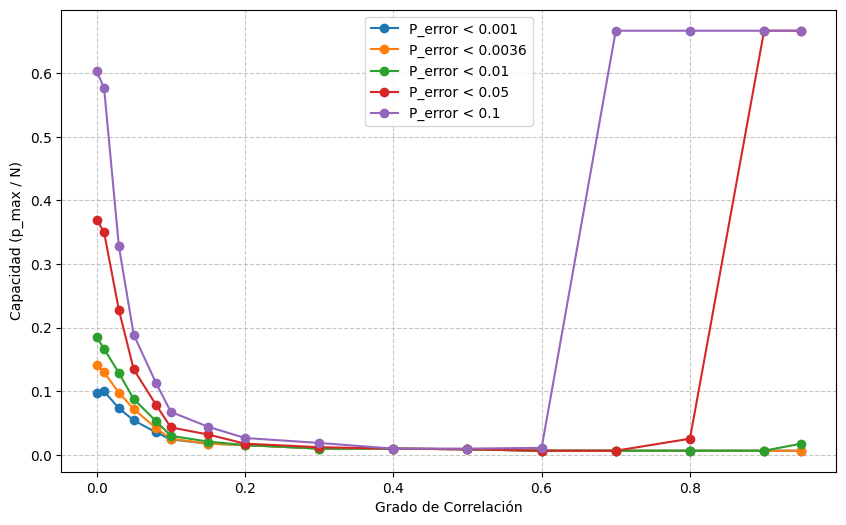
\includegraphics[width=0.7\textwidth]{img_informe/correlacion_capacidad.png}
	\caption{Relación entre correlación y capacidad de la red para distintos umbrales de error.}
	\label{fig:corr_vs_cap}
\end{figure}

